%\title{Template for a Thesis}
%%%%%%%%%%%%%%%%%%%%%%%%%%%%
% PREAMBLE OF THE DOCUMENT %
%%%%%%%%%%%%%%%%%%%%%%%%%%%%
%
%%%%%%%%%%%%%%%%%%%%%%%%%%%%%%%%%%%%%%%%%%%%%%%%%%%%%%%%%%%%%%%%
%
% 				         Edited by Nicola Rainiero
%				         http://rainnic.altervista.org/tag/latex
%			       	     ---------------------------------------
%%%%%%%%%%%%%%%%%%%%%%%%%%%%%%%%%%%%%%%%%%%%%%%%%%%%%%%%%%%%%%%%
%
% book - Default class for a normal book
\documentclass[a4paper,12pt,oneside,table]{book}

% extbook - a class for text bigger than 12pt
%\documentclass[a4paper,14pt,twoside,openright,reqno,table]{extbook}

% Options in detail:
% openany - allows chapter and similar openings to occur on left hand pages
% openright - allows chapter and similar openings to occur on right hand pages
% fleqn  - left-alignment of formulas
% leqno - labels formulas on the left-hand side instead of right
% reqno - labels formulas on the right-hand side
% draft - in draft mode the figures are not loaded, useful for speeding up typesetting
% onecolumn or twocolumn
% oneside (default for article and report)
% twoside (default for book)
% table  --> to avoid the message: package xcolor has already been loaded ...

\usepackage{packages}
% Almost all the settings are defined in packages.sty

% Put a grey textual watermark on document pages (PS mode only)
%\usepackage[italian,light,first,bottomafter]{draftcopy}

% Put a grey textual watermark on document pages (PDF mode)
%\usepackage{draftwatermark}
% If you want to change the default DRAFT text
%\SetWatermarkText{DRAFT}
% If you want to change the default grey color of the text
%\SetWatermarkColor{red}

%%%%%%%%%%%%%%%%%%%%%%%%%%%%%%%%%%%%%%%%%%%
%   DOCUMENT: an ordered list of files    %
%             that you can include or not %
%             in your document            %
%%%%%%%%%%%%%%%%%%%%%%%%%%%%%%%%%%%%%%%%%%%
\begin{document}

% Title Page %
% ====================== Centred Title Page ===========================

% \begin{titlepage}
% \thispagestyle{empty}
% \centering
% %\providecommand\pdfbookmark[3][]{} \pdfbookmark[0]{Title Page}{bm:Title}
% \vspace*{5cm}
% \textsc{\huge{First Line of Your Title}}\\[0.5em]
% \textsc{\huge{Second Line}}\\[0.5em]
% \textsc{\huge{Third}}\\[0.5em]
% \vfill
% By\\[0.5em]
% \textsc{\Large{Joseph Chamberlain}}
% \vfill
% A thesis submitted to\\[-0.8em]
% the University of Birmingham\\[-0.8em]
% for the  degree of\\[-0.8em]
% \MakeUppercase{Doctor of Philosophy} \\[\baselineskip]
% \begin{figure}[ht!]
% \begin{center}
% 
\includegraphics[height=4cm]{frontmatter/images/BirminghamUniversityCrest.png}
% \end{center}
% \end{figure}
% Cold Atoms Research Group\\[-0.8em]
% School of Physics and Astronomy\\[-0.8em]
% College of Engineering and Physical Sciences\\[-0.8em]
% University of Birmingham\\[-0.8em]
% September~2020 \\[\baselineskip]
% %\copyright\ Copyright by \MakeUppercase{\@Author},~\@Year\\
% %All Rights Reserved
% \end{titlepage}
% \clearpage

% ================ Aligned Title Page ===========================

\thispagestyle{empty}
\providecommand\pdfbookmark[3][]{} \pdfbookmark[0]{Title Page}{bm:Title}
\vspace*{1cm}
\begin{figure}[ht!]
    \centering
    
\includegraphics[height=4cm]{frontmatter/images/BirminghamUniversityCrest.png}
\end{figure}
\vfill
\begin{center}
    {\large{Mid-Course Assessment}}\\[1.0em]
    {\huge{Hierarchically Modelling Stars}}\\[0.5em]
    {\huge{Using Deep Learning and}}\\[0.5em]
    {\huge{Asteroseismology}}\\[0.5em]
    \vfill
    By\\[\baselineskip]
    {\Large{Alexander J. Lyttle}}
    \vfill
    \begin{tabular}{rl}
        \emph{Student ID} & 1532473\\[-0.8em]
        \emph{Supervisor} & Dr Guy R. Davies\\[-0.8em]
        \emph{Co-Supervisor} & Dr Andrea Miglio\\[-0.8em] 
    \end{tabular}
\end{center}
\begin{center}
    Solar and Stellar Physics Group\\[-0.8em]
    School of Physics and Astronomy\\[-0.8em]
    College of Engineering and Physical Sciences\\[-0.8em]
    University of Birmingham\\[1.0em]
    \today\\[\baselineskip]
\end{center}
%\copyright\ Copyright by \MakeUppercase{\@Author},~\@Year\\
%All Rights Reserved
\clearpage



%% FRONTMATTER %%
% The pages inside of frontmatter are in Roman numerals and the chapters will not have numeration
\frontmatter

% COPYRIGHT %
% ======================== Copyright page ===============================

\thispagestyle{empty}
%\providecommand\pdfbookmark[3][]{} \pdfbookmark[0]{Copyright}{bm:Copyright}
\addtocounter{page}{-1}
\vspace*{\fill}
\vfill
\begin{center}
\copyright\ Copyright by \MakeUppercase{Alexander J. Lyttle},~2020\\
All Rights Reserved
\end{center}
%\vspace{1in}
\clearpage

% ABSTRACT %
\providecommand\phantomsection{} \phantomsection
%\addcontentsline{toc}{part}{Abstract}
\thispagestyle{plain}
\begin{center}
%\hrule
\providecommand\pdfbookmark[3][]{} \pdfbookmark[0]{Abstract}{bm:Abstract}
% \vspace*{1in}
\textbf{ABSTRACT}\\[2\baselineskip]
% \vspace*{.1in}
\end{center}

% ========= Your Abstract Goes Here =========
\lipsum[1]


% % DEDICATION %
% % ======================= Dedication Page ============================
\newpage
\thispagestyle{plain}%
\begin{center}
%\providecommand\pdfbookmark[3][]{}\pdfbookmark[0]{DedicationPage}{bm:Dedicate}
\vspace*{1.575in}
\textbf{DEDICATION}\\[2\baselineskip]
I dedicate this to my Grandpa,\\
an inspirational man and talented violinist.\\
May he rest in peace\\
to the music of the stars.
\end{center}%
\vfill
\newpage


% ACKNOWLEDGEMENTS %
% ========================= Acknowledgments ==============================
\providecommand\phantomsection{} \phantomsection
%\addcontentsline{toc}{part}{Acknowledgments}
\thispagestyle{plain}
\renewcommand{\baselinestretch}{1}\small\normalsize
\begin{center}
%\providecommand\pdfbookmark[3][]{}\pdfbookmark[0]{Acknowledgments}{bm:Acknowledge}
\vspace*{0.375in}
\textbf{ACKNOWLEDGMENTS}\\[3\baselineskip]
\end{center}
\renewcommand{\baselinestretch}{1.66} \small\normalsize%
I acknowledge the people who helped me.
\newpage

% % CREDITS %
% \begin{titlepage}

\nonumber
\null \vspace {\stretch{1}}
%	\begin{flushright}
%	\begin{verse}
    \begin{center}
\textit{Worker bees can leave\\
even drones can leave\\
the queen is their slave} \\[5mm]
%	\end{verse}
	Tyler Durden, ''Fight Club''
%	\end{flushright}
    \end{center}
\vspace{\stretch{2}}\null

\end{titlepage}
\cleardoublepage

% CONTENTS %
% To help hyperref to jump to the correct page
\phantomsection
%\addcontentsline{toc}{chapter}{Contents}
\tableofcontents

\renewcommand{\cftpartfont}{\normalfont\bfseries} % \part font in ToC
\renewcommand{\cftchapfont}{\normalfont\bfseries} % \chapter font in ToC
\renewcommand{\cftchappagefont}{\normalfont}
\renewcommand{\cftpartpagefont}{\normalfont}
\renewcommand{\cftpartleader}{\cftdotfill{\cftdotsep}}
\renewcommand{\cftchapleader}{\cftdotfill{\cftdotsep}}
\renewcommand{\cftsecleader}{\cftdotfill{\cftdotsep}}
% \setcounter{tocdepth}{4}
% \setcounter{secnumdepth}{4}

\cftsetindents{chapter}{0in}{0.25in}
\cftsetindents{section}{0.25in}{0.35in}
\cftsetindents{subsection}{.6in}{0.5in}
\cftsetindents{subsubsection}{1.5in}{0.5in}

\setlength{\cftbeforepartskip}{.25em}
\setlength{\cftbeforechapskip}{.25em}
\setlength{\cftbeforesecskip}{-.5em}
\setlength{\cftbeforesubsecskip}{-.5em}

\addtocontents{toc}{~\hfill\textbf{Page}\par}
\thispagestyle{plain}

\clearpage

  % Make the list of figures
\listoffigures
\thispagestyle{plain}
\clearpage

 % Make the list of tables
\listoftables
\thispagestyle{plain}
\clearpage
 

 
 
% GLOSSARY %
\cleardoublepage
% To help hyperref to jump to the correct page
\phantomsection
% To add the Glossary in the table of contents
%\addcontentsline{toc}{chapter}{Glossary}
% Prints the glossary
\printglossary

% In order to update the glossary you have to execute:
% \makeindex -s main.ist -t main.alg -o main.acr main.acn
% to insert an item in the document:
% \newglossaryentry{item_label}{name={item}, description={description}}
% if it doesn't appear you have to initialize it:
% \glsadd{item_label}
% or if it is called again in the following text:
% \gls{item_label}

% ACRONYMS %
\cleardoublepage
% To help hyperref to jump to the correct page
\phantomsection
% To add the Index of Symbols in the table of contents
%\addcontentsline{toc}{chapter}{Acronyms}
% Prints the Acronyms
\printglossary[type=\acronymtype,title=Acronyms]

% In order to update the symbols you have to execute:
% makeindex -s main.ist -t main.glg -o main.gls main.glo
% to insert an item in the document::
% \newacronym{item_label}{name={item}, description={description}}
% if it doesn't appear you have to initialize it:
% \glsadd{item_label}
% or if it is called again in the following text:
% \gls{item_label}

%% MAINMATTER %%
% The pages inside of mainmatter are in Arabic numerals and the chapters will have numeration
\mainmatter

%\part{If you want parts}
\chapter{Introduction}

\section{Astroseismology}

\subsection{Solar-like oscillators}

\subsection{Detecting oscillation modes}

\subsection{Helium II Ionization Zone Glitch}

\section{Machine Learning in Astrophysics}

\section{Hierarchical Bayesian Models in Astrophysics}

\section{Open-Source Code in Astrophysics}

\chapter{Peakbagging with \texttt{PBjam}}

\section{How it Works}

\section{Contributing to the Code}

\section{Peakbagging with TESS}

\chapter{Hierarchically Modelling Many Stars}

See the accompanying paper (Appendix \ref{apx:paper}).

% Preface with some sections elaborating or explaining certain things.

\chapter{Future Work}\label{ch:future}

\section{Including the Helium II Glitch}

\section{Increasing the Sample Size}

\section{To Higher Mass Stars and Beyond}

Our next step is to include intermediate-mass stars with masses from approx. 1.2 solar masses to 3.0 solar masses.


%% APPENDICES %%
\appendix
\chapter{Accompanying Paper}\label{apx:paper}
\vspace*{-0.3in}

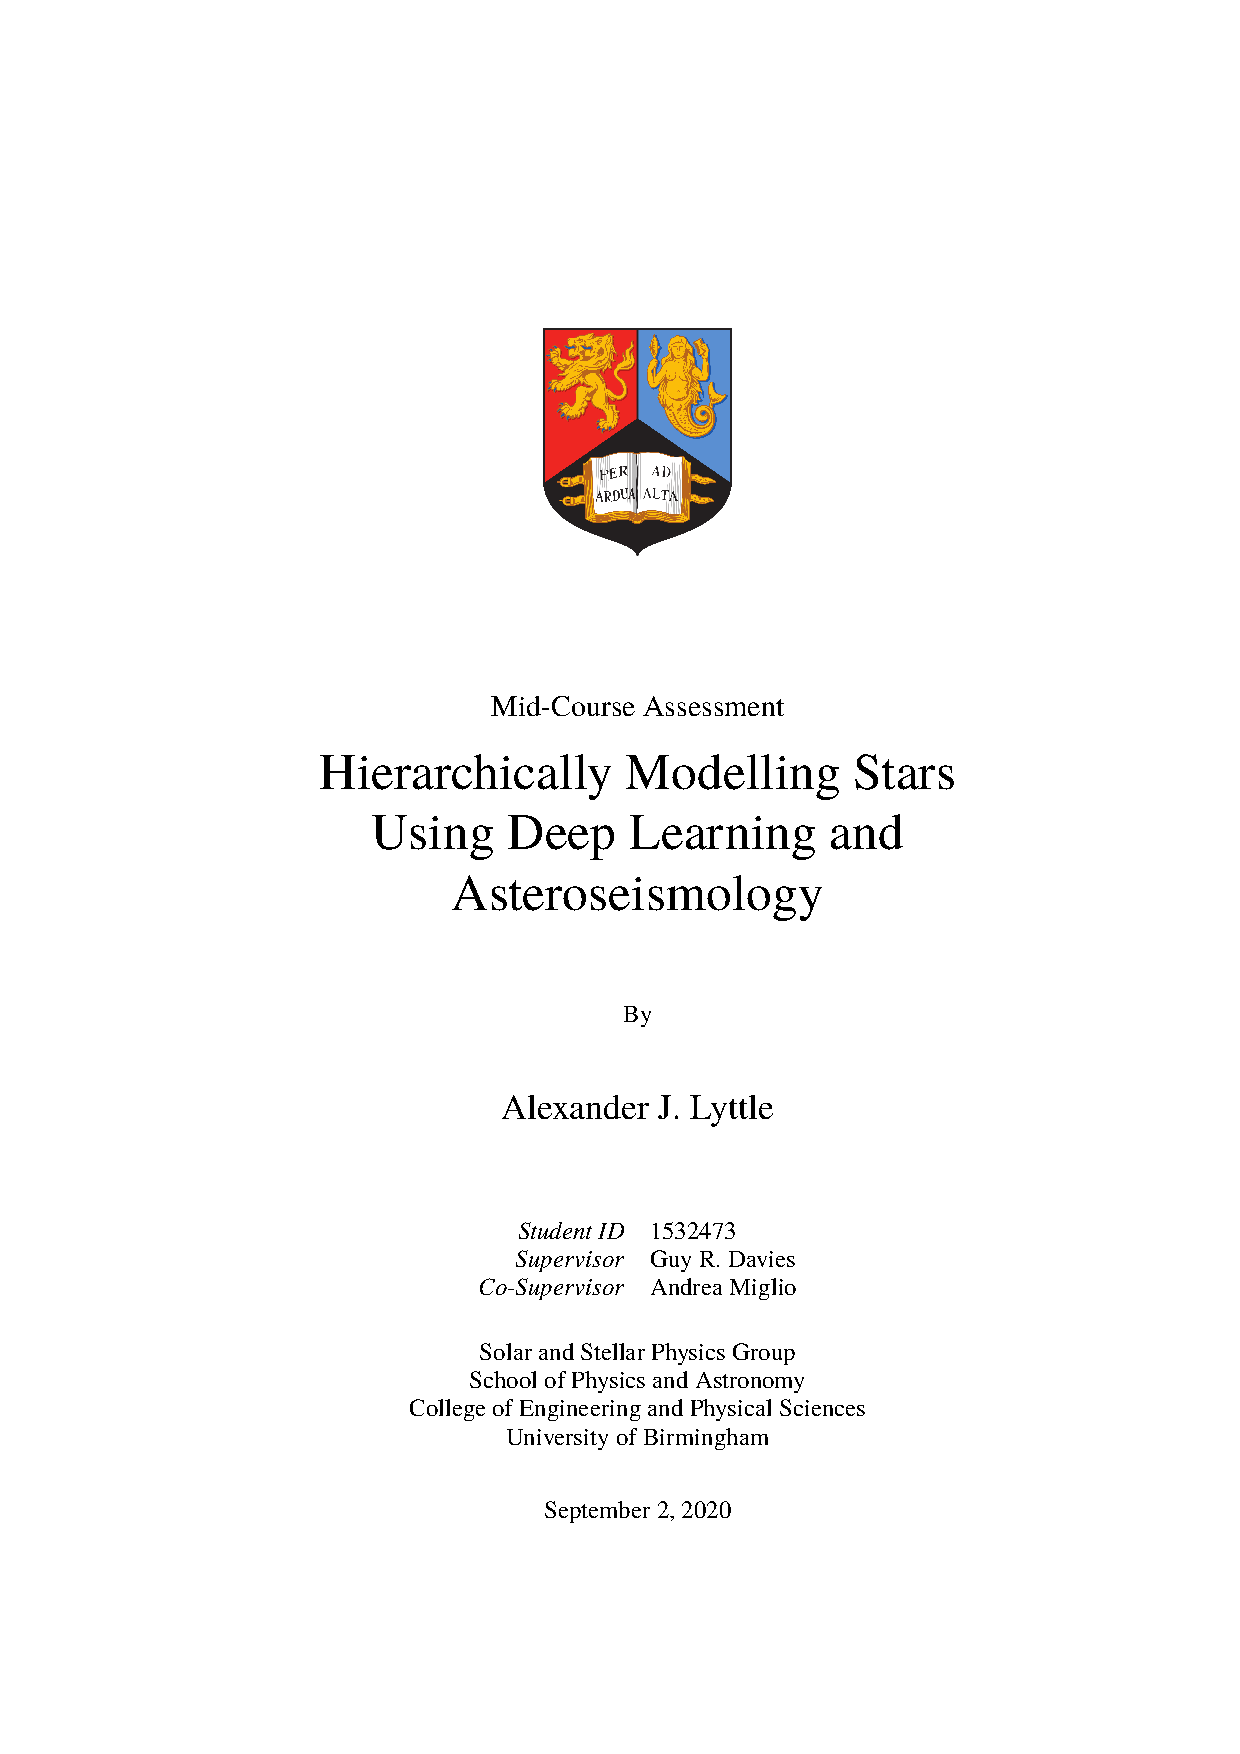
\includepdf[pages=-]{../kepler-dwarfs/paper/main.pdf}


%% BACKMATTER %%
% The pages inside of backmatter are in Arabic numerals and the chapters will not have numeration
\backmatter

% BIBLIOGRAPHY WITH BIBTEX %
%*******************************************************
% Bibliography
%*******************************************************
\cleardoublepage
\phantomsection
\addcontentsline{toc}{part}{References}
\printbibliography[title=References]
% \bibliographystyle{../mnras}
% \bibliography{../bibliography}
\nocite{*}
% \vspace{2.5cm}
% \begin{Large}Websites consulted\end{Large}
% \begin{itemize}
% \item Wikipedia -- \url{www.wikipedia.org}
% \end{itemize}


% All the sources are described in a file named bibliography.bib
% if you want to cite one in the text:
% \citep{label}
% In order to update the bibliography you have to execute:
% bibtex main (without ".tex")

% INDEX %
\cleardoublepage
% To help hyperref to jump to the correct page
\phantomsection
% To add the Index in the table of contents
\addcontentsline{toc}{chapter}{Index}
% Prints the Index
\printindex
% To add an item in it, write the \index{WORD} after the word to highlight:
% WORD\index{WORD}
% In order to update the Index you have to execute:
% makeindex main (without ".tex")

% A typical session involving a bibliography, an index and so on would require:
% pdflatex main
% makeindex -s main.ist -t main.alg -o main.acr main.acn
% makeindex -s main.ist -t main.glg -o main.gls main.glo
% bibtex main
% pdflatex main
% pdflatex main
% makeindex main
% makeindex -s main.ist -t main.alg -o main.acr main.acn
% makeindex -s main.ist -t main.glg -o main.gls main.glo
% pdflatex main
% pdflatex main
\end{document}